Once we analyzed the results for each of the projects, we had a closer look at the different errors and create a taxonomy that could be used for any Java project and answering \textbf{RQ2}.

As we mentioned in the methodology chapter (See Chapter \ref{subsec:taxonomy}), we will use the taxonomy development method of Nickerson et al.~\cite{Nickerson2013}. The objective of this chapter, therefore, will be to classify the errors obtained from the failed builds.

First step in this methodology is to define a meta-characteristic, a starting point to define the characteristics of our taxonomy. Each characteristic should be a logical consequence of the metacharacteristic. In our case, the meta-characteristic will be \textit{the nature of the fail}. 

The objects that we will use for the development of the taxonomy were the errors obtained in the previous phase (what we called symptoms), a total of 86 errors from the 6 subject proyects. These errors have been randomly divided into 5 groups of 17-18 errors. All data needed and the detailed process are available in a public repository~\footnote{\url{https://github.com/Maes95/TFM-Buildability/tree/ReproducePackage/Taxonomy}}. Detailed steps to reproduce the taxonomy are available in Appendix~\ref{apx:taxonomy-steps}

Five iterations have been carried out using the method, the results of which are shown below. 

\begin{enumerate}%[\bfseries {I}ter{a}t{i}on 1]
	
	%\vspace{3mm}
	\item For this iteration a \textit{conceptual-to-empirical} approach has been used, using as a starting point a previous taxonomy, \textit{Build Errors: A Case Study}~\cite{Seo:2014:PBE:2568225.2568255}, from which we take the types of errors \textit{Semantic} (Not override a superclass or interface method when use override annotation, incompatible types, not suitable method \dots), \textit{Syntax} (keywords expected, illegal start of expression, statement expected, parsing XML files~\dots) and \textit{Dependency} (can not import this package, could not resolve a library or a version of it \dots), which are common in Java projects. Since these types do not cover all objects, it is necessary to switch to an empirical approach and add two new types: \textit{Encoding} (using bad encoder for strings) and \textit{Build System} (any problem related to de execution of the build system technology). The taxonomy resulting from this iteration is: \textit{$T_{1}$ = {Type(Build System, Dependency, Encoding, Semantic, Syntax)}}.
	
	\vspace{2mm}
	\item For this iteration a \textit{empirical-to-conceptual} approach has been used. In this iteration, all objects are classified with the current taxonomy, so there is no need to expand it. The taxonomy resulting from this iteration is: \textit{$T_{2}$ = {Type(Build System, Dependency, Encoding, Semantic, Syntax)}}.
	
	\vspace{2mm}
	\item For this iteration a \textit{conceptual-to-empirical} approach has been used. When no new types are detected in last iteration, the use of another dimension of the objects is explored. In the development of an application, we can find that we have made mistakes in the source code, in the configuration or the error is external. This new dimension, the location, could take the following values: Source code, config files or external. Applying this new dimension on the objects of this iteration, all are classified within the domain of the new dimension. No new types arise. The taxonomy resulting from this iteration is: \textit{$T_{3}$ = {Type(Build System, Dependency, Encoding, Semantic, Syntax), Location(Source code, Config files, External) }}.
	
	\vspace{2mm}
	\item For this iteration a \textit{empirical-to-conceptual} approach has been used. From the logs of this iteration, we find that the taxonomy is insufficient and it is necessary to extend it. The type Enviroment (problems in the execution environment) is added. The taxonomy resulting from this iteration is: \textit{$T_{4}$ = {Type(Build System, Dependency, Encoding, Enviroment, Semantic, Syntax), Location(Source code, Config files, External) }}.
	
	\vspace{2mm}
	\item For this iteration a \textit{empirical-to-conceptual} approach has been used. In this iteration, all objects are classified with the current taxonomy, so there is no need to expand it. The taxonomy resulting from this iteration is: \textit{$T_{5}$ = {Type(Build System, Dependency, Encoding, Enviroment, Semantic, Syntax), Location(Source code, Config files, External) }}.
\end{enumerate}          

In figure~\ref{fig:taxonomyTree} we can see the final taxonomy. The classification of the errors made is summarised by project in table \ref{table:taxonomyResults}.

% \begin{figure}[h!]
% 	\begin{center}
% 		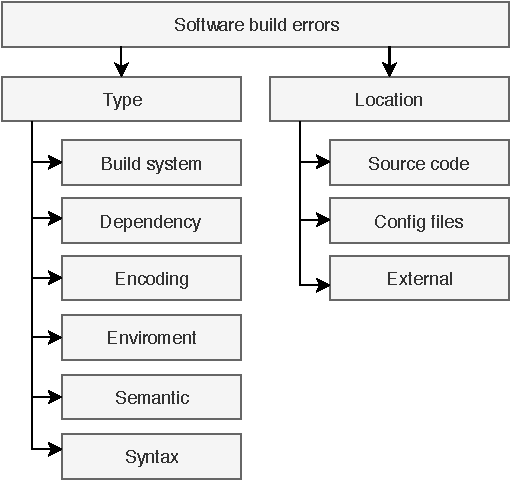
\includegraphics[width=11cm]{img/Taxonomy}
% 		\caption{Developed taxonomy of software build errors}
% 		\label{fig:taxonomyTree}
% 	\end{center}
% \end{figure}

\begin{table*}
	\caption{Taxonomy results}
	\label{table:taxonomyResults}
	\centering
	\begin{tabular}{>{\rowmac}r>{\rowmac}r>{\rowmac}r>{\rowmac}r>{\rowmac}r>{\rowmac}r>{\rowmac}r>{\rowmac}r<{\clearrow}}
		\setrow{\bfseries} & CLOSURE & LANG    & MATH    & MOCKITO & SPRING  & TIME     & Average \\
		\toprule
		\setrow{\bfseries}
		Build system & 33.33\% & 91.15\% & 94.41\% & 98.62\% & 61.18\% & 100.00\% & 79.78\%        \\
		\midrule
		Config Files & 0.00\%  & 0.06\%  & 0.00\%  & 21.42\% & 1.93\%  & 0.00\%   & 3.90\%         \\
		External     & 33.33\% & 91.09\% & 94.41\% & 77.20\% & 59.25\% & 100.00\% & 75.88\%        \\
		\midrule
		\setrow{\bfseries}
		Dependency   & 33.33\% & 0.30\%  & 0.00\%  & 0.95\%  & 9.55\%  & 0.00\%   & 7.36\%         \\
		\midrule
		Config Files & 0.00\%  & 0.30\%  & 0.00\%  & 0.67\%  & 5.69\%  & 0.00\%   & 1.11\%         \\
		External     & 0.00\%  & 0.00\%  & 0.00\%  & 0.00\%  & 0.36\%  & 0.00\%   & 0.06\%         \\
		Source Code  & 33.33\% & 0.00\%  & 0.00\%  & 0.29\%  & 3.50\%  & 0.00\%   & 6.19\%         \\
		\midrule
		\setrow{\bfseries}
		Encoding     & 0.00\%  & 6.58\%  & 0.00\%  & 0.00\%  & 1.78\%  & 0.00\%   & 1.39\%         \\
		\midrule
		Source Code  & 0.00\%  & 6.58\%  & 0.00\%  & 0.00\%  & 1.78\%  & 0.00\%   & 1.39\%         \\
		\midrule
		\setrow{\bfseries}
		Enviroment   & 0.00\%  & 0.00\%  & 0.00\%  & 0.00\%  & 20.70\% & 0.00\%   & 3.45\%        \\
		\midrule
		External     & 0.00\%  & 0.00\%  & 0.00\%  & 0.00\%  & 20.70\% & 0.00\%   & 3.45\%        \\
		\midrule
		\setrow{\bfseries}
		Semantic     & 33.33\% & 1.85\%  & 5.59\%  & 0.43\%  & 6.78\%  & 0.00\%   & 8.00\%         \\
		\midrule
		Source Code  & 33.33\% & 1.85\%  & 5.59\%  & 0.43\%  & 6.78\%  & 0.00\%   & 8.00\%         \\
		\midrule 
		\setrow{\bfseries}
		Syntax       & 0.00\%  & 0.12\%  & 0.00\%  & 0.00\%  & 0.02\%  & 0.00\%   & 0.02\%         \\
		\midrule
		Config Files & 0.00\%  & 0.06\%  & 0.00\%  & 0.00\%  & 0.00\%  & 0.00\%   & 0.01\%         \\
		Source Code  & 0.00\%  & 0.06\%  & 0.00\%  & 0.00\%  & 0.02\%  & 0.00\%   & 0.02\%        
	\end{tabular}
\end{table*}

\vspace{0.3cm}
\begin{tcolorbox}[fonttitle=\bfseries,title=Answer to RQ2: What are the most common problems that cause
	snapshot build fail?,label=rq2,colframe=blue!50!black]
	Considering the taxonomy made and the errors classified in it, we can conclude that the most common errors we find when building the snapshot of a Java project are due to the Build System (79.78\%), to the semantics of the language (8.00\%) and to the dependencies of the project (7.36\%). Other less common errors are related to the environment (3.45\%), encoding (1.39\%) and syntax (0.02\%).
\end{tcolorbox}
